\subsubsection{Descripción y topología de los paquetes}

Nuestro segundo experimento consistió en capturar los paquetes de la LAN Wi-Fi de la empresa Honeywell. En esta red no hay mucho tráfico, ya que la mayoría de las computadores se conectan via Ethernet a una VPN. Esta red es dedicada a transacciones que no necesiten un nivel de seguridad. La captura se realizo un día lunes a las 11 am. durante media hora, lográndose capturar 253 paquetes.  

\begin{figure}[H]
 \begin{center}
  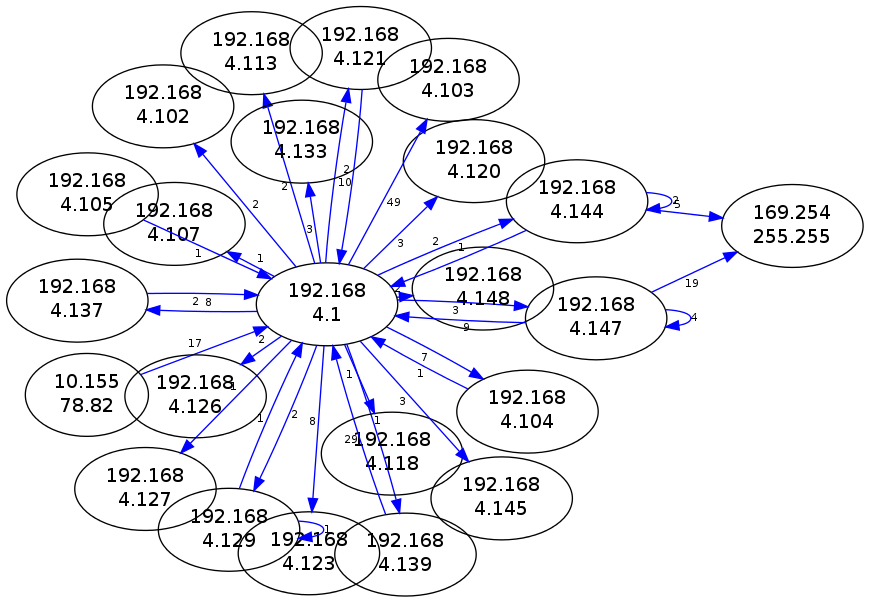
\includegraphics[width=0.7\linewidth]{../imgs/red-honeywell_red.png}
  \caption{Medición Honeywell}
 \end{center}
\end{figure}


\subsubsection{Fuente: $S_{dst}$}

\begin{figure}[H]\centering
    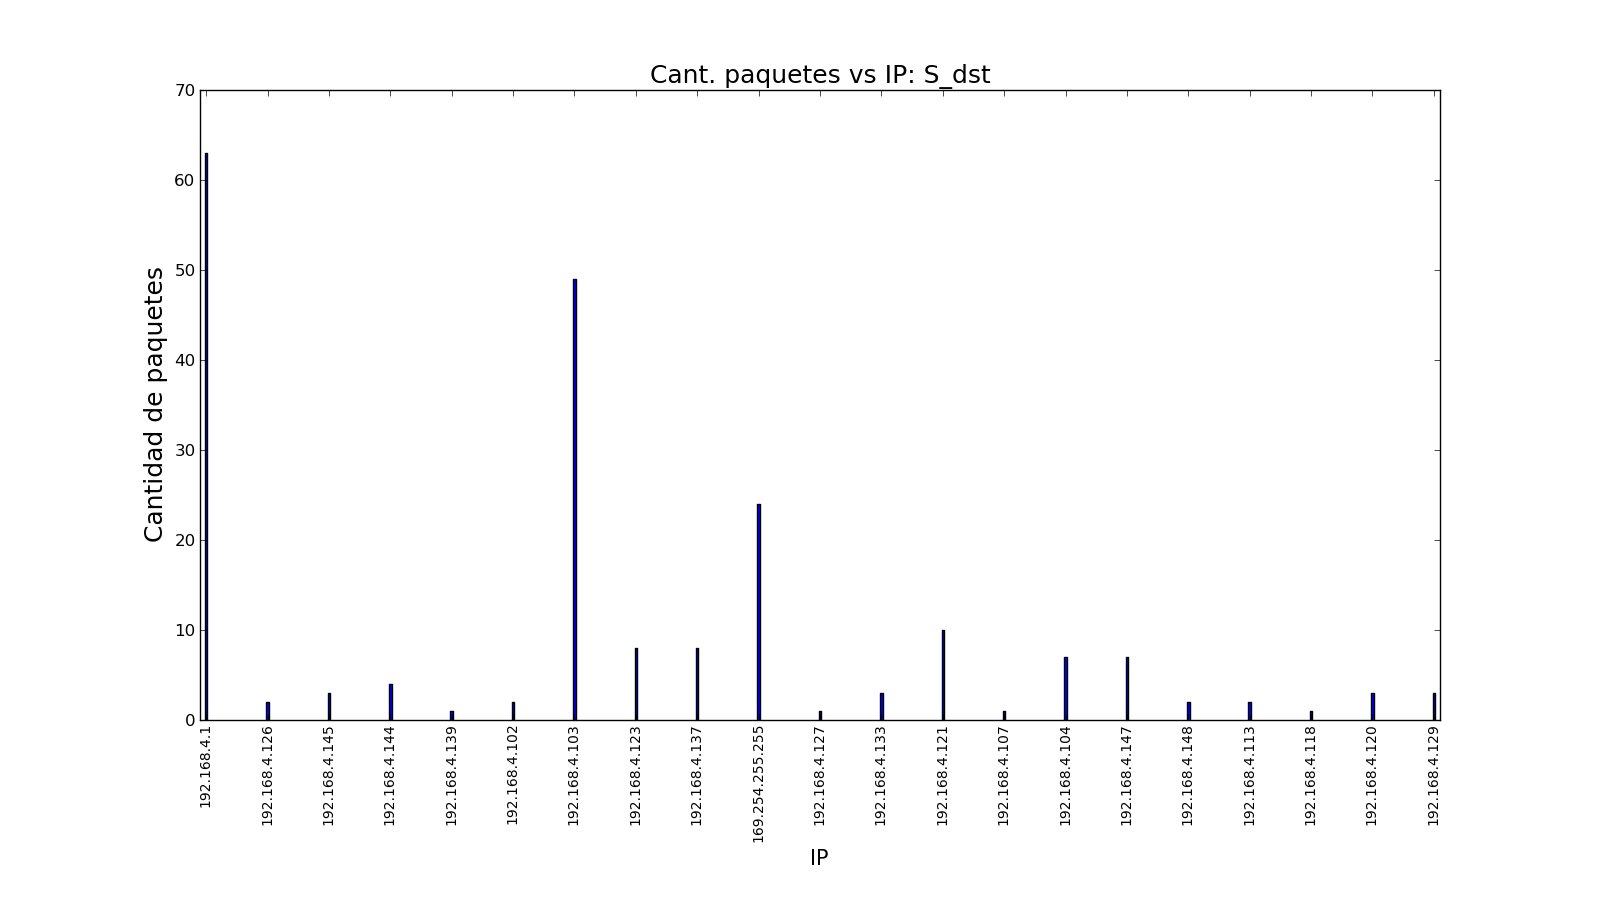
\includegraphics[width=0.8\linewidth]{../imgs/red-honeywell_S_dst_hist.png}
    \caption{Histograma de $S_{dst}$}\label{fig:Honeywell-dst-hist}
\end{figure}

\begin{figure}[H]\centering
    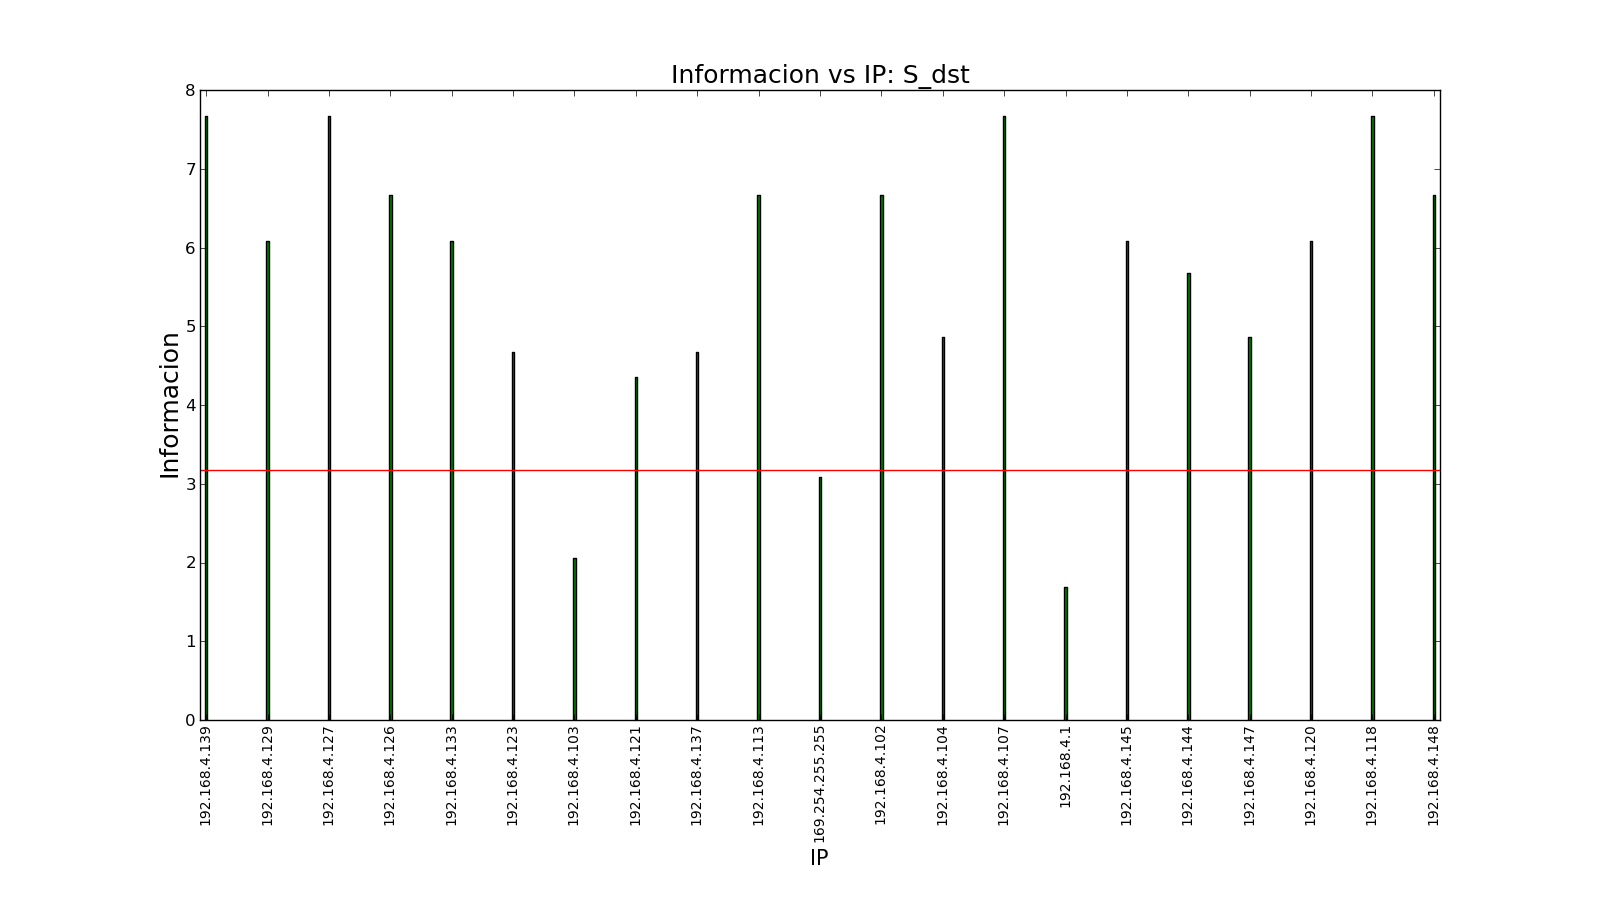
\includegraphics[width=0.8\linewidth]{../imgs/red-honeywell_S_dst_info.png}
    \caption{Informacion de $S_{dst}$}\label{fig:Honeywell-dst-info}
\end{figure}

$\bullet$ Entropía de la fuente: 3.17600221734

\subsubsection{Fuente: $S_{src}$}

\begin{figure}[H]\centering
    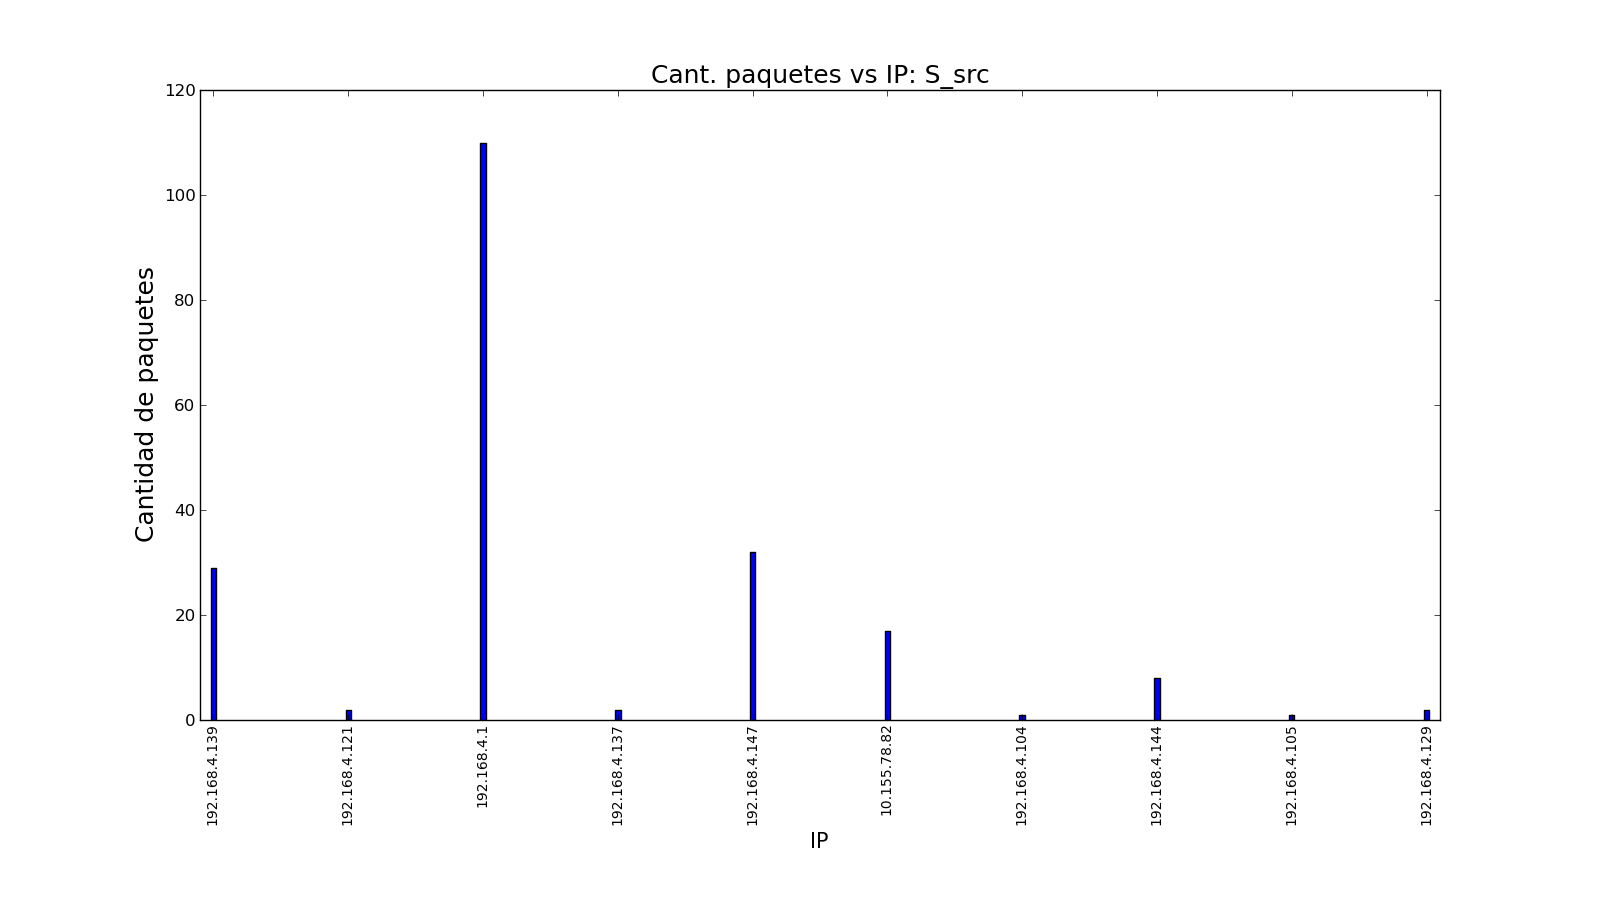
\includegraphics[width=0.8\linewidth]{../imgs/red-honeywell_S_src_hist.png}
    \caption{Histograma de $S_{src}$}\label{fig:Honeywell-src-hist}
\end{figure}

\begin{figure}[H]\centering
    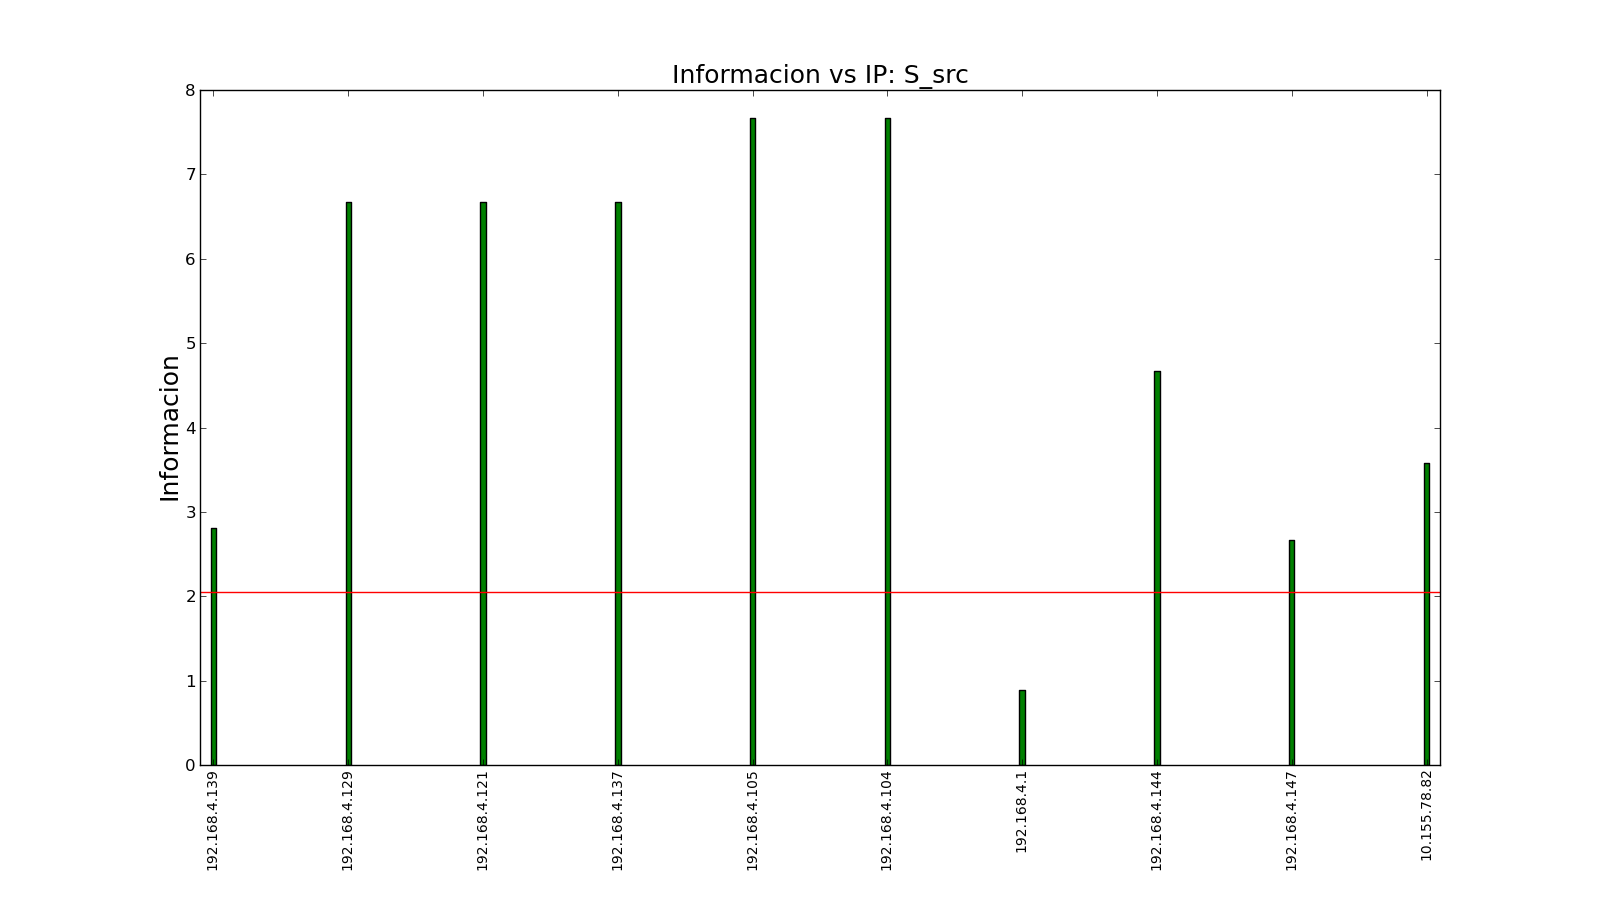
\includegraphics[width=0.8\linewidth]{../imgs/red-honeywell_S_src_info.png}
    \caption{Informacion de $S_{src}$}\label{fig:Honeywell-src-info}
\end{figure}

$\bullet$ Entropía de la fuente: 2.05322002017

\subsubsection{Discusión}

cualquier cosa interesante sobre este caso en particular